\documentclass{article}
\usepackage{amsfonts,amssymb,amsmath,amsthm}

%% set-style letters
\def\AA{{\mathbb{A}}}
\def\BB{{\mathbb{B}}}
\def\CC{{\mathbb{C}}}
\def\DD{{\mathbb{D}}}
\def\EE{{\mathbb{E}}}
\def\FF{{\mathbb{F}}}
\def\GG{{\mathbb{G}}}
\def\HH{{\mathbb{H}}}
\def\II{{\mathbb{I}}}
\def\JJ{{\mathbb{J}}}
\def\KK{{\mathbb{K}}}
\def\LL{{\mathbb{L}}}
\def\MM{{\mathbb{M}}}
\def\NN{{\mathbb{N}}}
\def\OO{{\mathbb{O}}}
\def\PP{{\mathbb{P}}}
\def\QQ{{\mathbb{Q}}}
\def\RR{{\mathbb{R}}}
\def\SS{{\mathbb{S}}}
\def\TT{{\mathbb{T}}}
\def\UU{{\mathbb{U}}}
\def\VV{{\mathbb{V}}}
\def\WW{{\mathbb{W}}}
\def\XX{{\mathbb{X}}}
\def\YY{{\mathbb{Y}}}
\def\ZZ{{\mathbb{Z}}}

%% calligraphic letters
\def\cA{{\mathcal{A}}}
\def\cB{{\mathcal{B}}}
\def\cC{{\mathcal{C}}}
\def\cD{{\mathcal{D}}}
\def\cE{{\mathcal{E}}}
\def\cF{{\mathcal{F}}}
\def\cG{{\mathcal{G}}}
\def\cH{{\mathcal{H}}}
\def\cI{{\mathcal{I}}}
\def\cJ{{\mathcal{J}}}
\def\cK{{\mathcal{K}}}
\def\cL{{\mathcal{L}}}
\def\cM{{\mathcal{M}}}
\def\cN{{\mathcal{N}}}
\def\cO{{\mathcal{O}}}
\def\cP{{\mathcal{P}}}
\def\cQ{{\mathcal{Q}}}
\def\cR{{\mathcal{R}}}
\def\cS{{\mathcal{S}}}
\def\cT{{\mathcal{T}}}
\def\cU{{\mathcal{U}}}
\def\cV{{\mathcal{V}}}
\def\cW{{\mathcal{W}}}
\def\cX{{\mathcal{X}}}
\def\cY{{\mathcal{Y}}}
\def\cZ{{\mathcal{Z}}}
\def\cKL{{\mathcal{KL}}}

%% bold letters
\def\bA{{\bf{A}}}
\def\bB{{\bf{B}}}
\def\bC{{\bf{C}}}
\def\bD{{\bf{D}}}
\def\bE{{\bf{E}}}
\def\bF{{\bf{F}}}
\def\bG{{\bf{G}}}
\def\bH{{\bf{H}}}
\def\bI{{\bf{I}}}
\def\bJ{{\bf{J}}}
\def\bK{{\bf{K}}}
\def\bL{{\bf{L}}}
\def\bM{{\bf{M}}}
\def\bN{{\bf{N}}}
\def\bO{{\bf{O}}}
\def\bP{{\bf{P}}}
\def\bQ{{\bf{Q}}}
\def\bR{{\bf{R}}}
\def\bS{{\bf{S}}}
\def\bT{{\bf{T}}}
\def\bU{{\bf{U}}}
\def\bV{{\bf{V}}}
\def\bW{{\bf{W}}}
\def\bX{{\bf{X}}}
\def\bY{{\bf{Y}}}
\def\bZ{{\bf{Z}}}
\def\ba{{\bf{a}}}
\def\bb{{\bf{b}}}
\def\bc{{\bf{c}}}
\def\bd{{\bf{d}}}
\def\be{{\bf{e}}}
\def\boldf{{\bf{f}}} %different
\def\bg{{\bf{g}}}
\def\bh{{\bf{h}}}
\def\bi{{\bf{i}}}
\def\bj{{\bf{j}}}
\def\bk{{\bf{k}}}
\def\bl{{\bf{l}}}
\def\bm{{\bf{m}}}
\def\bn{{\bf{n}}}
\def\bo{{\bf{o}}}
\def\bp{{\bf{p}}}
\def\bq{{\bf{q}}}
\def\br{{\bf{r}}}
\def\bs{{\bf{s}}}
\def\bt{{\bf{t}}}
\def\bu{{\bf{u}}}
\def\bv{{\bf{v}}}
\def\bw{{\bf{w}}}
\def\bx{{\bf{x}}}
\def\by{{\bf{y}}}
\def\bz{{\bf{z}}}

%% other symbols
\DeclareMathOperator{\1}{\mathbf{1}}
\DeclareMathOperator{\0}{\mathbf{0}}
\DeclareMathOperator{\Id}{I}
\newcommand{\td}{\mathfrak{t}} % discrete-time 
\newcommand{\tr}{^\top}

%% operators
\DeclareMathOperator{\col}{col}
\DeclareMathOperator{\diag}{diag}
\DeclareMathOperator{\blkdiag}{blkdiag}
\DeclareMathOperator{\rank}{rank}
\DeclareMathOperator{\dis}{d}
\DeclareMathOperator{\sat}{sat} 
\DeclareMathOperator{\convhull}{\textbf{co}}
\DeclareMathOperator{\argmin}{argmin}
\DeclareMathOperator{\argmax}{argmax}
\DeclareMathOperator{\spec}{spec}
\def\He#1{\texttt{\rm{He}}\left\{{#1}\right\}}
\DeclareMathOperator{\trace}{tr}
\newcommand{\Imag}{\mathrm{Im}}

%% shortcuts
\newcommand{\norm}[1]{\lvert #1\rvert}
\newcommand{\wnorm}[2]{\lvert #1\rvert^2_{#2}}
\newcommand{\pderiv}[2]{\dfrac{\partial #1}{\partial #2}}
\newcommand{\pdef}[1]{\SS_{\succ0}^{#1}}
\newcommand\psemidef[1]{\SS_{\succeq0}^{#1}}
\newcommand{\bmx}[1]{\left[\begin{matrix}#1\end{matrix}\right]}
\newcommand{\pmx}[1]{\left(\begin{matrix}#1\end{matrix}\right)}
\newcommand{\smallpmat}[1]{\left(\begin{smallmatrix} #1 \end{smallmatrix} \right)}
\newcommand{\smallqmat}[1]{\left[\begin{smallmatrix} #1 \end{smallmatrix} \right]}
\newcommand{\overbar}[1]{\mkern 1.5mu\overline{\mkern-1.5mu#1\mkern-1.5mu}\mkern 1.5mu}
\renewcommand{\underbar}[1]{\mkern 1mu\underline{\mkern-1mu#1\mkern-1mu}\mkern 1mu}

\usepackage{hyperref}
\usepackage{graphicx}
\usepackage{float}

% SCRIPTS FOR DOUBLE AND SINGLE IMAGE

% \begin{figure}[H]
%     \centering
%     \begin{subfigure}{0.4\textwidth}
%     \includegraphics[width=\textwidth]{}
%     \caption{}
%     \label{}
%     \end{subfigure}
%     \hfill
%     \begin{subfigure}{0.55\textwidth}
%     \includegraphics[width=\textwidth]{}
%     \caption{}
%     \label{}
%     \end{subfigure}
%     \caption{}
%     \label{}
% \end{figure}

% \begin{figure}[H]
%     \centering
%     \includegraphics[width=0.65\textwidth]{}
%     \caption{}
%     \label{}
% \end{figure}

\usepackage[margin=54pt]{geometry}
\usepackage{biblatex}
\addbibresource{biblio.bib}


\begin{document}

\date{Theory recap}
\author{Marco Sterlini}

\title{Title}
\maketitle

\section*{First works}
My contribution started by exploring the works \cite{css-paper} and \cite{css-extended}. The problem addressed is the design of an event-triggered control (ETC) for discrete-time linear-time-invariant (LTI) systems.
The aim was to decrease the computational load that follows the application of non-linear activation functions inside the neural network (NN) controller. Also thanks to previous works \cite{sophie-book-saturation}, \cite{arcak-first}, \cite{iqc-intro} several tools to treat these non-linearities have been studied and applied allowing the use of classical stability analysis methods to highly non-linear NN controllers. Lyapunov theory will be used to guarantee the stability of the NN controlled plant.

\subsection*{System under analysis}

The feedback system under examination is the following:

\begin{figure}[H]
    \centering
    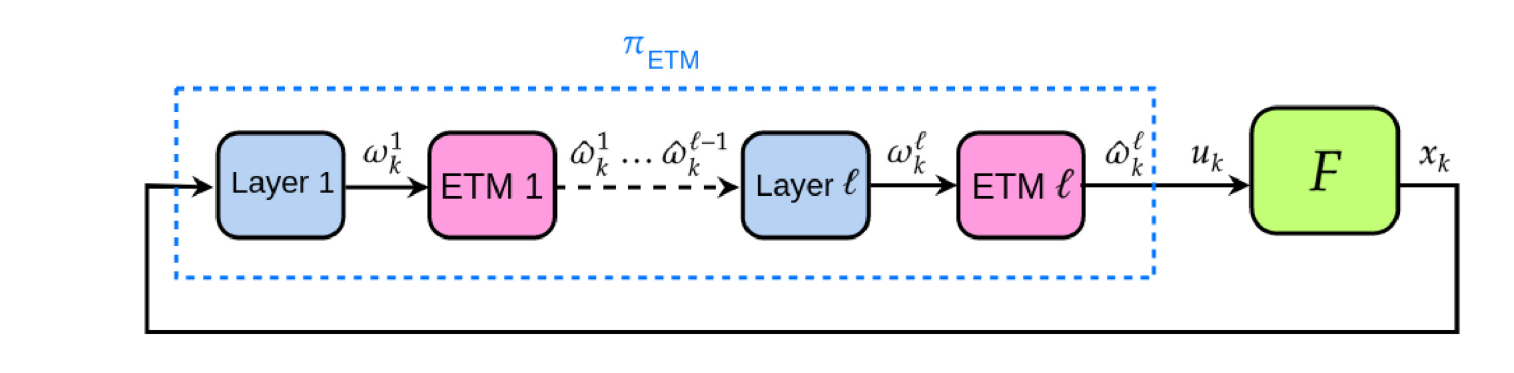
\includegraphics[width=0.6\textwidth]{img/simple-etm}
    \label{}
\end{figure}

The NN controller is called $\pi_{ETM}$, the plant to stabilize is $F$, and it is described by the dynamics:

\begin{align*}
    &x(k + 1) = A_{F} x(k) + B_{F} u(k)\\
    \\
    &\hat{\omega}^{0}(k) = x(k),\\
    &\nu^{i}(k) = W^{i} \hat{\omega}^{i-1}(k) + b^{i},\ \ i \in \left\{ 1, \dots, l \right\},\\
    &\omega^{i}(k) = \text{sat}(\nu^{i}(k)),\\
    &u(k) = W^{l+1} \hat{\omega}^{l} (k) + b^{l+1}\\ 
\end{align*}

Where the first equation describes the plant $F$ as a discrete-time linear time-invariant system, the other equations describe the behavior of the NN controller: $\hat{\omega}^{i}$ and $\omega^{i}$ are respectively the last and current output of the $i^{th}$ layer, $\nu^{i}$ is the current input to the $i^{th}$ layer. The control input $u(k)$ is hence the output of the last layer of the NN, also the weights and the biases of the $i^{th}$ layer are indicated by $W^{i}$ and $b^{i}$. As per the activation function the saturation function was used and is defined by:
$$
   \text{sat}(\nu^{i}_{j}(k)) = \text{sign}(\nu^{i}_{j}(k)) min(|\nu^{i}_{j}(k)|, \bar{\nu}^{i}_{j})
$$  
For the $j^{th}$ neuron of the $i^{th}$ layer where $\bar{\nu}^{i}_{j}$ is the relative maximum limit value for the input signal. The activation function is applied element wise but a notation to isolate the non-linearities is used:
$$
    \nu_{\phi} = \bmx{\nu^{1\tr}, \dots \nu^{l\tr}}\tr, \omega_{\phi} = \bmx{\omega^{1\tr}, \dots \omega^{l\tr}}\tr, \hat{\omega}_{\phi} = \bmx{\hat{\omega}^{1\tr}, \dots \hat{\omega}^{l\tr}}\tr \in \RR^{n_{\phi}}
$$
With $n_{\phi}$ the total number of neurons involved in the controller. It is then possible to express:
$$
    \text{sat}(v_{\phi}) = \bmx{\text{sat}(\nu^{1})\tr, \dots, \text{sat}(\nu^{l})\tr}\tr \in \RR^{n_{\phi}}
$$
The control input $u(k)$ and the input layers' vector $\nu_{\phi}$ can be expressed as a function of the state $x(k)$ and the last layers' output vector $\hat{\omega}_{\phi}(k)$

\begin{equation}
    \bmx{u(k)\\ \nu_{\phi}(k)} = \bmx{\begin{array}{c|cccc|c} 
        \0 & \0 & \dots & \0 & W^{l+1} & b^{l+1}\\
        \hline
        W^{1} & \0 & \dots & \0 & \0 & b^{1}\\
        \0 & W^{2} & \dots & \0 & \0 & b^{2}\\
        \vdots & \vdots & \ddots & \vdots & \vdots & \vdots\\
        \0 & \0 & \dots & W^{l} & \0 & b^{l}
    \end{array}}  \bmx{x(k) \\ \hat{\omega}_{\phi}(k) \\ 1}
\end{equation}

$$
    \bmx{u(k)\\ \nu_{\phi}(k)} = N  \bmx{x(k) \\ \hat{\omega}_{\phi}(k) \\ 1}\text{ and } N = \bmx{N_{ux} & N_{u \omega} & N_{ub} \\ N_{vx} & N_{v \omega} & N_{vb}}
$$

Then the equilibrium point $\left( x_{*}, u_{*}, \nu_{*}, \omega_{*} \right)$ is computed.

\subsection*{ETM definition}
Different approaches were used in \cite{css-paper} and \cite{css-extended}, the first work takes into account the difference between the input and output vectors of the network at different time instants, the latter instead directly uses the sector conditions as the triggering ones.

\pagebreak
\printbibliography


\end{document}